\subsubsection{応用:GIF アニメーションの作成}
\label{GIF}
gif アニメーションを使ってスライドショー作ってみましょう。gif とは画像ファイルのフォーマットの 1 つで、アニメーションを表現することもできます。\\
\begin{enumerate}
\item ディレクトリ slideshow を/home/pi に作りましょう。\\
\item スライドショーの素材(パラパラ漫画の一枚一枚)を集めます。インターネットで画像を検索したり、Gimp で作ったりしましょう。画像は今作った slideshow というディレクトリに保存しましょう。\\
\item 画像の名前が連番になるように名前を変更します。00.jpg 01.jpg 02.jpg … のようにスライドショーで表示したい順番の番号を名前にしましょう。\\
\begin{figure}[H]
    \centering
    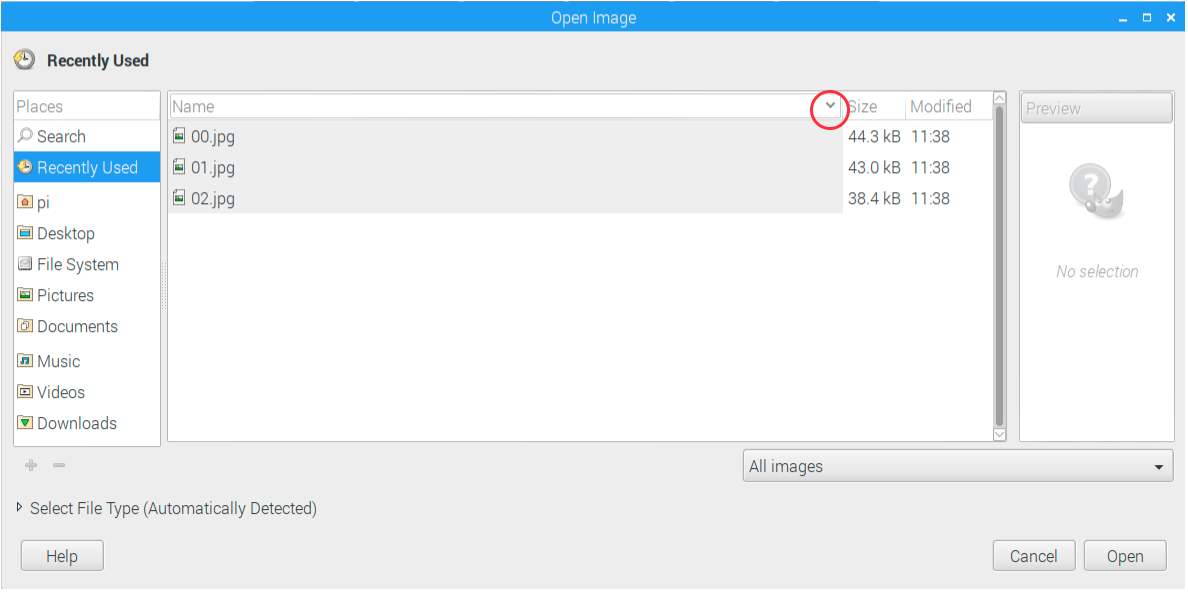
\includegraphics[width=\linewidth]{images/chap03/text03-img025.png}
\end{figure}
\item Gimp を開きます。「ファイル」→「開く/インポート」で「画像ファイルを開く」ウィンドウを出し、最初の一枚目を選択して開きます。Gimp で「ファイル」→「レイヤーとして開く」で、2 番め以降の全てのファイルを選択して開きましょう。Shift キーを押しながらクリックすることで複数選択できます。選択するときは、「名前」をクリックして名前の順に並び替えておきましょう。\\
\item Gimp で「ファイル」→「名前をつけてエクスポート」をクリックします。名前をslideshow.gif とし、エクスポートボタンを押します。
\begin{figure}[H]
    \centering
    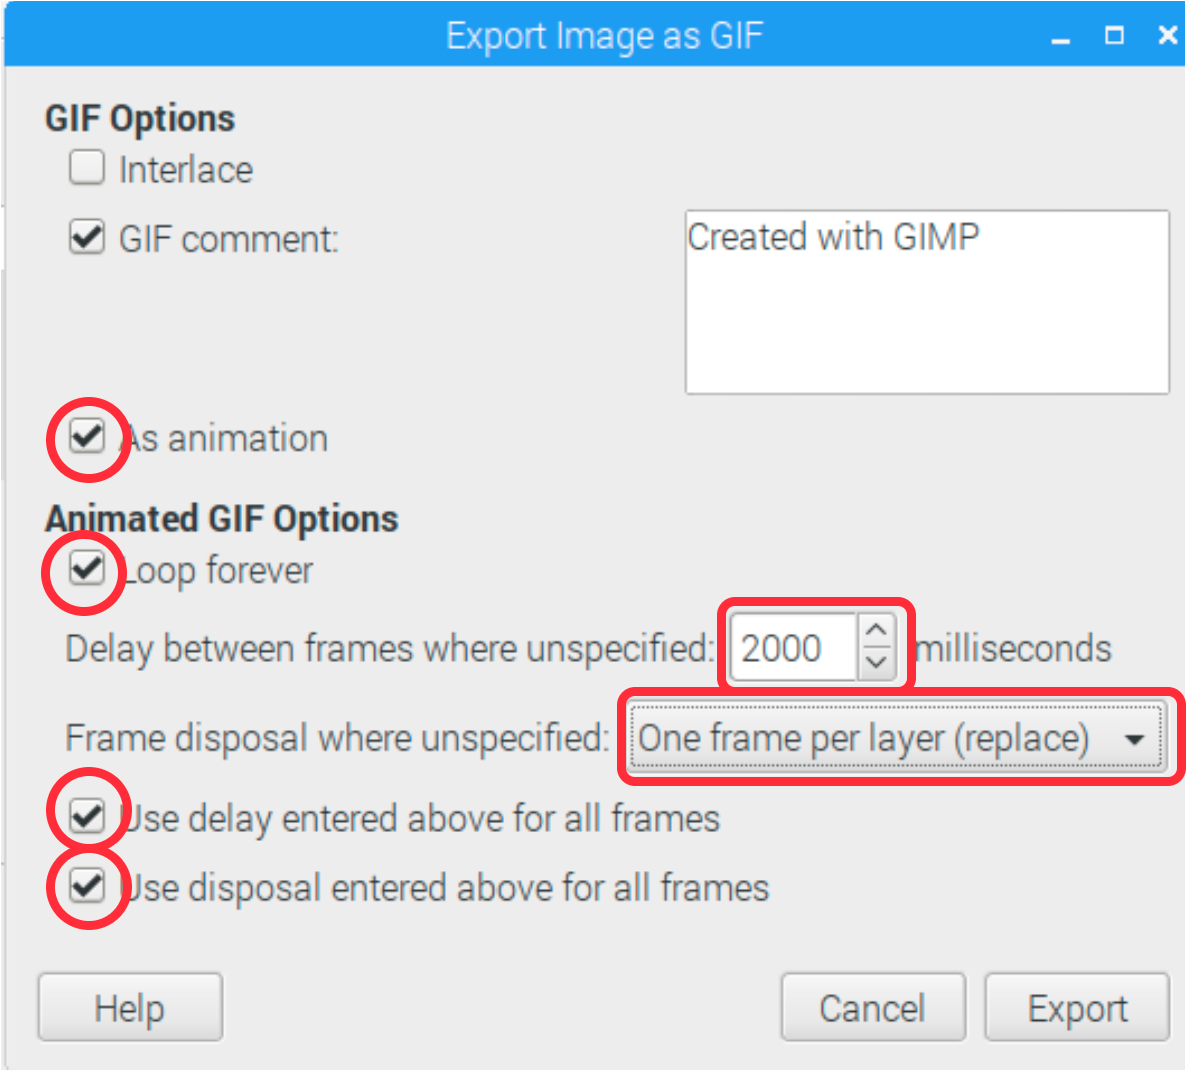
\includegraphics[width=0.6\linewidth]{images/chap03/text03-img026.png}
\end{figure}
\item 「画像をエクスポート: GIF 形式」というウィンドウが出るので、「アニメーションとしてエクスポート」にチェック、「指定しない場合のディレイ」をお好みに(2000 ミリ秒くらいがオススメ)、「指定しない場合のフレーム処理」を「レイヤーごとに 1 フレーム(置換)」に、「全フレームのディレイにこの値を使用」にチェック、「全フレームのフレーム処理にこの値を使用」にチェックをしてエクスポートボタンを押します。\\
\item 出来上がった画像をみてみましょう。下記どちらかのコマンドでみることができます。\\
chromium-browser slideshow.gif\\
gpicview slideshow.gif\\
\end{enumerate}

\begin{tcolorbox}[title=\useOmetoi]
%\begin{minipage}{0.94\hsize}
\begin{enumerate}
\item \ref{GIF}を見ながら、オリジナルのアニメーションを作成しましょう。
\end{enumerate}
%\end{minipage}
\end{tcolorbox}